%! TEX TS-program = xelatex
\documentclass[a4paper,10pt]{article}
\usepackage{geometry}
\usepackage{lipsum}
\usepackage{fancyhdr}
\usepackage{fontspec}
\usepackage{setspace}
\usepackage{ulem}
\usepackage{indentfirst}
\usepackage[english, russian]{babel}
\usepackage[hidelinks]{hyperref}
\usepackage{graphicx}
\usepackage{amsmath}
\usepackage{totcount}
\usepackage{calc}

 \graphicspath{ {./images/} }

\setmainfont{Times New Roman}

\usepackage{fontspec}
\newcommand{\arial}{\fontspec{Arial}}
\usepackage{tikz}
\newcommand{\mainframe}[9]{
	\itshape
	\small
	\arial
	\begin{tikzpicture}[remember picture, overlay]

		\draw[black, ultra thick]

		([shift={(20mm, 5mm)}] current page.south west)
		--
		([shift={(20mm, -5mm)}] current page.north west)
		--
		([shift={(-5mm, -5mm)}] current page.north east)
		--
		([shift={(-5mm, 5mm)}] current page.south east)
		-- cycle;
		\draw[black, ultra thick]
		([shift={(20mm, 45mm)}] current page.south west)
		--
		([shift={(-5mm, 45mm)}] current page.south east)
		([shift={(20mm, 35mm)}] current page.south west)
		--
		++(65mm, 0)
		([shift={(20mm, 30mm)}] current page.south west)
		--
		([shift={(-5mm, 30mm)}] current page.south east)
		++(0, -5mm)
		--
		+(-50mm, 0)
		++(0, -5mm)
		--
		+(-50mm, 0)

		([shift={(20mm, 45mm)}] current page.south west)
		++(7mm, 0)
		--
		+(0mm, -15mm)
		++(10mm, 0)
		--
		+(0, -40mm)
		++(23mm, 0)
		--
		+(0, -40mm)
		++(15mm, 0)
		--
		+(0, -40mm)
		++(10mm, 0)
		--
		+(0, -40mm)

		([shift={(-5mm, 30mm)}] current page.south east)
		++(-20mm, 0)
		--
		+(0, -10mm)
		++(-15mm, 0)
		--
		+(0, -10mm)
		++(-15mm, 0)
		--
		+(0, -25mm);

		\draw[black, thick]
		([shift={(-5mm, 30mm)}] current page.south east)
		++(-40mm, -5mm)
		--
		+(0, -5mm)
		++(-5mm, 0)
		--
		+(0, -5mm);
		\draw[black, thick]
		([shift={(20mm, 5mm)}] current page.south west)
		++(0, 5mm)
		--
		+(65mm, 0)
		++(0, 5mm)
		--
		+(65mm, 0)
		++(0, 5mm)
		--
		+(65mm, 0)
		++(0, 5mm)
		--
		+(65mm, 0)
		++(0, 15mm)
		--
		+(65mm, 0);
		\draw[anchor=mid]
		([shift={(20mm, 35mm)}] current page.south west)
		++(0, -2.7mm)
		+(3.5mm, 0)
		node {Изм.}

		+(12mm, 0)
		node {Лист}

		+(28.5mm, 0)
		node {№ докум.}

		+(47.5mm, 0)
		node {Подп.}

		+(60mm, 0)
		node {Дата}

		+(8.5mm, -5mm)
		node [
				text width = 15mm,
				align = left
			] {Разраб.}

		+(8.5mm, -10mm)
		node [
				text width = 15mm,
				align = left
			]{Пров.}

		+(8.5mm, -15mm)
		node [
				text width = 15mm,
				align = left
			] {Реценз.}

		+(8.5mm, -20mm)
		node [
				text width = 15mm,
				align = left
			] {Н. контр.}

		+(8.5mm, -25mm)
		node [
				text width = 15mm,
				align = left
			] {Утв.}





		([shift={(-5mm, 30mm)}] current page.south east)
		++(0, -2.7mm)
		+(-10mm, 0)
		node {Листов}

		+(-27.5mm, 0)
		node {Лист}

		+(-42.5mm, 0)
		node {Литера}

		++(0, -5mm)
		+(-10mm, 0)
		node {#9}

		+(-27.5mm, 0)
		node {#8}
		;


		\draw[anchor=mid]
		([shift={(37mm, 30mm)}] current page.south west)

		+(11.5mm, -2.7mm)
		node [
				text width = 21mm,
				align = left
			] {#4}

		+(11.5mm, -7.7mm)
		node [
				text width = 21mm,
				align = left
			] {#5}

		+(11.5mm, -17.7mm)
		node [
				text width = 21mm,
				align = left
			] {#6}

		+(11.5mm, -22.7mm)
		node [
				text width = 21mm,
				align = left
			] {#7}
		;

		%\upshape
		\huge
		\draw
		([shift={(-5mm, 30mm)}] current page.south east)
		+(-60mm, 7.5mm)
		node {#1}
		;

		\large
		\draw
		([shift={(-5mm, 5mm)}] current page.south east)
		+(-25mm, 7.5mm)
		node [
				anchor = center,
				text width = 50mm,
				align = center
			]{#2}
		;

		\large
		\draw
		([shift={(-55mm, 5mm)}] current page.south east)
		+(-35mm, 12.5mm)
		node [
				anchor = center,
				text width = 70mm,
				align = center
			]{#3}
		;

	\end{tikzpicture}
}




\newcommand{\pageframe}[2]{
	\itshape
	\small
	\arial
	\begin{tikzpicture}[remember picture, overlay]

		\draw[black, ultra thick]

		([shift={(20mm, 5mm)}] current page.south west)
		--
		([shift={(20mm, -5mm)}] current page.north west)
		--
		([shift={(-5mm, -5mm)}] current page.north east)
		--
		([shift={(-5mm, 5mm)}] current page.south east)
		-- cycle;
		\draw[black, ultra thick]
		([shift={(20mm, 20mm)}] current page.south west)
		--
		([shift={(-5mm, 20mm)}] current page.south east)

		([shift={(20mm, 10mm)}] current page.south west)
		--
		+(65mm, 0)

		([shift={(-5mm, 5mm)}] current page.south east)
		+(0, 8mm) -- +(-10mm, 8mm)
		+(-10mm, 0) -- +(-10mm, 15mm)

		([shift={(20mm, 5mm)}] current page.south west)
		++(7mm, 0) -- +(0, 15mm)
		++(10mm, 0) -- +(0, 15mm)
		++(23mm, 0) -- +(0, 15mm)
		++(15mm, 0) -- +(0, 15mm)
		++(10mm, 0) -- +(0, 15mm)
		;

		\draw[black, thick]
		([shift={(20mm, 15mm)}] current page.south west)
		-- +(65mm, 0)
		;

		\draw[anchor=mid]
		([shift={(20mm, 5mm)}] current page.south west)
		++(0, 2.3mm)
		+(3.5mm, 0)
		node {Изм.}

		++(7mm, 0)
		+(5mm, 0)
		node {Лист}

		++(10mm, 0)
		+(11.5mm, 0)
		node {№ докум.}

		++(23mm, 0)
		+(7.5mm, 0)
		node {Подп.}

		++(15mm, 0)
		+(5mm, 0)
		node {Дата}

		([shift={(-5mm, 13mm)}] current page.south east)
		+(-5mm, 3.3mm)
		node {Лист}
		;

		\normalsize
		\draw
		([shift={(-10mm, 9mm)}] current page.south east)
		node {#2}
		;

		\huge
		\draw
		([shift={(85mm, 5mm)}] current page.south west)
		+(55mm, +7.5mm)
		node {#1}
		;

	\end{tikzpicture}
}

\usepackage{tocloft}

\renewcommand{\cftsecleader}{\cftdotfill{\cftdotsep}}
\renewcommand{\cftdotsep}{1}

\setlength{\cftbeforesecskip}{0.5em}
\setlength{\cftbeforesubsecskip}{0.5em}

\setlength{\cftsecnumwidth}{7mm}
\setlength{\cftsubsecnumwidth}{10mm}


% Изменение стилей названий разделов
\usepackage{titlesec}

\setcounter{secnumdepth}{4}

\titleformat{\section}[block]{\hspace{\parindent}}{\thesection}{1em}{}
\titleformat{\subsection}[block]{\hspace{\parindent}}{\thesubsection}{1em}{}
\titleformat{\subsubsection}[block]{\hspace{\parindent}}{\thesubsubsection}{1em}{}
\titleformat{\paragraph}[block]{\hspace{\parindent}}{\theparagraph}{1em}{}


\titlespacing{\section}{0pt}{2em}{2em}
\titlespacing{\subsection}{0pt}{2em}{2em}
\titlespacing{\subsubsection}{0pt}{2em}{2em}
\titlespacing{\paragraph}{0pt}{2em}{2em}

\newcommand{\topic}{Разработка конструктора Telegram-ботов. Часть 1}
\newcommand{\authorsn}{Бушков}
\newcommand{\authori}{
	\authorsn~Б. Д.}
\newcommand{\tpga}{TПЖА.09.03.01.514~ПЗ}


\newcommand{\docparindent}{12.5mm}


\newcommand{\csection}[1]{
	{
			\titleformat{\section}[block]{\centering}{\thesection}{1em}{}
			\phantomsection
			\section*{#1}
			\addcontentsline{toc}{section}{#1}
		}
}

\usepackage{caption}

\DeclareCaptionLabelSeparator{custom}{ -- }
\DeclareCaptionLabelFormat{flformat}{Рисунок #2}
\DeclareCaptionLabelFormat{tlformat}{Таблица #2}


\captionsetup[figure]{
	font=Large,
	labelsep=custom,
	labelformat=flformat,
	justification=centering,
	margin=1cm
}


\captionsetup[table]{
	format=plain,
	font=Large,
	labelsep=custom,
	labelformat=tlformat,
	singlelinecheck=false,
	margin={\docparindent, 0pt},
	skip=0.5em,
}

% Изменение стилей списков

\usepackage{enumitem}



\newcommand{\labelv}{--}
% Отступ от label у itemize
\newcommand{\ilabelsep}{0.5em}
% Отступ от label y enumerate, level 1
\newcommand{\eilabelsep}{0.5em}
% Отступ от label у enumarate, level 2
\newcommand{\eiilabelsep}{0em}


\setlist[itemize]{
	itemsep=0pt,
	parsep=0pt,
	topsep=0pt,
	labelsep=\ilabelsep,
	label=\labelv,
	itemindent=\parindent+\ilabelsep+\labelwidth,
	leftmargin=0pt,
	align=left,
}


\setlist[enumerate,1]{
	label=\arabic*),
	ref=\arabic*,
	align=left,
	itemsep=0pt,
	parsep=0pt,
	topsep=0pt,
	labelwidth=\widthof{99)},
	labelsep=\eilabelsep,
	leftmargin=\parindent+\labelwidth+\labelsep,
}

\setlist[enumerate,2]{
	label=\theenumi.\arabic*),
	align=left,
	itemsep=0pt,
	parsep=0pt,
	topsep=0pt,
	labelsep=\eiilabelsep,
	labelwidth=\widthof{99.99)},
	leftmargin=\labelwidth+\labelsep,
}




%\renewcommand{\cftchapleader}{\cftdotfill{\cftdotsep}}
\geometry{top = 15mm, left = 25mm, right = 10mm, bottom = 15mm}

\renewcommand{\headrulewidth}{0pt}
\fancypagestyle{mainframe} {
    \fancyhf{}
    \fancyhead[L]{
        \mainframe
        {\tpga}
        {Кафедра ЭВМ Группа ИВТ-41}{
        \topic
        }
        {\authori}
        {Долженкова}
        {Скворцов}
        {Долженкова}
        {\thepage}
        {\total{page}}
    }

}
\fancypagestyle{pageframe} {
    \fancyhf{}
    \fancyhead[L]{
        \pageframe
        {\tpga}
        {\thepage}
    }
}

\onehalfspacing
\setlength{\parindent}{12.5mm}


\sloppy
\regtotcounter{page}
\regtotcounter{equation}


\begin{document}
\renewcommand{\contentsname}{\hfill Содержание \hfill}
\Large
\pagestyle{empty}
\begin{titlepage}
	\newpage
	\singlespacing
	\topskip = 0.8cm
	\large
	%\setlength{\ULdepth}{1.8pt}

	\begin{center}
		\large
		%\fontsize{11pt}{13pt}
		\bfseries
		МИНИСТЕРСТВО НАУКИ И ВЫСШЕГО ОБРАЗОВАНИЯ РФ \\
		ФЕДЕРАЛЬНОЕ ГОСУДАРСТВЕННОЕ БЮДЖЕТНОЕ \\
		ОБРАЗОВАТЕЛЬНОЕ УЧРЕЖДЕНИЕ ВЫСШЕГО ОБРАЗОВАНИЯ \\
		«ВЯТСКИЙ ГОСУДАРСТВЕННЫЙ УНИВЕРСИТЕТ» \\
		ИНСТИТУТ МАТЕМАТИКИ И ИНФОРМАЦИОННЫХ СИСТЕМ \\
		ФАКУЛЬТЕТ АВТОМАТИКИ И ВЫЧИСЛИТЕЛЬНОЙ ТЕХНИКИ \\
		КАФЕДРА ЭЛЕКТРОННЫХ ВЫЧИСЛИТЕЛЬНЫХ МАШИН
	\end{center}

	\vspace{0.8cm}
	\begin{center}
		\textbf{Направление}
		\uline{09.03.01 - Информатика и вычислительная техника}

		\small
		\textit{(код и наименование направления)}

		\large
		Профиль – \uline{Программное и аппаратное обеспечение вычислительной техники}
	\end{center}

	\vspace{0.8cm}
	\begin{flushright}
		Допускаю к защите \\
		Заведующий кафедрой ЭВМ \\
		\vspace{1mm}
		\uline{\hspace{3cm}} / \uline{Долженкова М.Л.} / \\
		\vspace{1mm}
		\small
		\itshape
		(подпись) \hspace{1.8cm} (Ф.И.О.) \hspace{1.4cm}

	\end{flushright}

	\vspace{1.5cm}
	\begin{center}
		\huge
		\bfseries
		\topic
	\end{center}

	\vspace{0.5cm}
	\begin{center}
		Пояснительная записка выпускной квалификационной работы \\
		\tpga
	\end{center}

	\newcommand{\ulinesize}{2.5cm}

	\large
	\vspace{1cm}
	\noindent
	Разработал: студент гр.ИВТб-4301-04-00 \hfill \uline{\hspace{\ulinesize}}
	/ \uline{\authori} / \hspace{8mm} \uline{\hspace{\ulinesize}}

	\vspace{1.5cm}
	\noindent
	Руководитель: к.т.н., доцент
	\hfill \uline{\hspace{\ulinesize}}
	/ \uline{Долженкова М. Л.} / \uline{\hspace{\ulinesize}}

	\vspace{1.5cm}
	\noindent
	Нормоконтролер: к.т.н., доцент кафедры ЭВМ
	\hfill \uline{\hspace{\ulinesize}}
	/ \uline{Скворцов А. А.} / \hspace{4mm} \uline{\hspace{\ulinesize}}

	{
		\small
		\itshape
		\hfill
		(подпись) \hspace{1.6cm} (Ф.И.О) \hspace{2.2cm} (дата) \hspace{0.8cm}
	}

	\begin{center}
		\vfill
		Киров \the\year
		\vspace{1cm}
	\end{center}


\end{titlepage}



{

\topskip = 0.8cm
\begin{center}
	Реферат
\end{center}

\vspace{1em}

\authori\
\topic
:\
\mbox{\tpga}\
ВКР / ВятГУ, каф. ЭВМ; рук.
Долженкова М.Л. – Киров, \the\year. –
Гр.ч. 8 л. ф.А1;
ПЗ \pageref{lastpage} с.,
1 рис.,
1 табл.,
1 источников,
1 прил.

\vspace{1.5em}

КОНСТРУКТОР,
TELEGRAM-БОТ,
КЛИЕНТСКАЯ ЧАСТЬ,
ВИЗУАЛЬНЫЙ РЕДАКТОР,
СЕРВЕРНАЯ ЧАСТЬ,
HTTP,
GOLAND,
POSTGRESQL,
TYPESCRIPT,
SOLID.JS,
JSON,
HTML,
CSS.

\vspace{1.5em}

Объект выпускной квалификационной работы -
конструктор ботов, представляющий собой
программное средство для упрощения
создания и управления ботами.

Целью данной выпускной квалификационной работы является повышение
скорости разработки, настройки и управления
ботами, что позволит пользователям
без специальных навыков
программирования создавать
эффективных ботов для различных целей.

Результат работы - разработка и реализация
конструктора Telegram-ботов,
который будет предоставлять
набор инструментов и
функций для создания и настройки
ботов, а также предоставлять
возможности для их управления.

}


\addtolength{\textheight}{-40mm}
\tocloftpagestyle{mainframe}
\pagestyle{pageframe}
\addtolength{\textheight}{+25mm}
\tableofcontents\newpage


\csection{Введение}

В современном мире стали популярными такие приложения для
быстрого общения как мессенджеры. Таких приложений достаточно много, но
большинство пользователей сети интернет все чаще отдают предпочтение
мессенджеру Telegram как наиболее удобному и надежному.

У Telegram имеется удобное API для создания ботов. Бот способен
выполнять определенные команды, заданные пользователем через интерфейс
Telegram. Данный функционал вполне может удовлетворять потребности
компании в предоставлении некоторых услуг в разных сферах. Например,
спортивные залы являются одной из таких сфер.

Создание ботов — это трудоемкий процесс, требующий
квалифицированных программистов, что довольно затратно для бизнеса.

Для решения данной проблемы существуют конструкторы Telegram-ботов, которые
предоставляют функции создания, редактирования и управления ботами.
К сожалению, большинство таких конструкторов предоставляют ограниченный функционал
при бесплатном использовании, а также имеют закрытые
способы хранения данных клиентов. Поэтому было принято решение выполнить анализ и
разработать конструктор Telegram-ботов без данных недостатков.





\section{Анализ предметной области}


На данном этапе работы необходимо рассмотреть функции
конструкторов Telegram-ботов,
провести обзор существующих на данный момент аналогов, рассмотреть их возможности,
выявить их
недостатки и обосновать актуальность разработки нового конструктора.

\subsection{Telegram-боты и конструкторы}

Боты в мессенджере Telegram становятся все более популярными и
число их пользователей постоянно растет. Они помогают пользователям
выполнять типичные рутинные действия в автоматизированном режиме,
значительно упрощая им жизнь. Для владельцев же самих ботов они стали
незаменимыми помощниками в работе.

Telegram-боты имеют множество плюсов, таких как:
\begin{itemize}
	\item круглосуточный доступ;
	\item моментальный ответ на запрос пользователя;
	\item удобство использования, интуитивно понятный интерфейс;
	\item не требуется установка дополнительных программ,
	      общение с ботом ведется через мессенджер.
\end{itemize}

Telegram-бот используют в коммерческой деятельности для следующих сфер и задач:
\begin{itemize}
	\item развлечения;
	\item поиск и обмен файлами;
	\item предоставление новостей;
	\item утилиты и инструменты;
	\item интеграция с другими сервисами;
	\item осуществление онлайн-платежей.
\end{itemize}


С популярностью ботов стали появляться все больше различных
конструкторов, которые позволяют
без наличия специальных знаний и
навыков создать своего бота всего в несколько кликов.

Конструктором называется NoCode инструмент, который
предназначен для
быстрого создания ботов без знания каких-либо языков программирования.
Иными словами, весь процесс создания – это нажатие тех или иных кнопок и
ввода текста (например, название кнопки, текст сообщения и т.д.).

Первое предназначение – упрощение работы. Ведь не все обладают
глубокими знаниями и навыками программирования. Когда боты только
появились, их могли разрабатывать только программисты, обладающие
соответствующим опытом и навыками.

Помимо того, что конструкторы позволяют расширить аудиторию,
способную создавать Telegram-ботов, они экономят время разработчикам. При
наличии конструктора нет необходимости разрабатывать каждый раз
отдельное приложение для выполнения типовых
задач, так как конструктор предоставляет необходимый
набор инструментов для быстрого создания бота
без необходимости писать код.

Но у конструкторов есть некоторые ограничения, например, при их
использовании нельзя выйти за рамки возможностей самого конструктора, а
также при выходе нового функционала Telegram API, его реализация в
конструкторе происходит с некоторой задержкой. Кроме того, боты,
реализованные с помощью NoCode решения обычно менее производительные,
чем их аналоги, написанные языке программирования.



\subsection{Обзор аналогов}

В подпунктах данного раздела рассматриваются существующие аналоги.
В качестве рассматриваемых аналогов были выбраны приложения,
реализующие функционал создания Telegram ботов с помощью конструктора.


\subsubsection{Бот-платформа «ManyBot»}


Один из наиболее популярных конструкторов. Работает внутри мессенджера Telegram.
Он бесплатный и прост в использовании.
Бот предоставляет создание бота с такими возможностями:
\begin{itemize}
	\item отправка сообщений;
	\item создание меню;
	\item автопостинг из VK, Twitter, YouTube;
	\item поддержка нескольких языков.
\end{itemize}

Минусы конструктора состоят в том, что нет администрирования
бота за пределами мессенджера, наличие рекламного сообщения в
созданном боте, малое количество компонентов и их модификаций,
а также отсутствие статистических данных по созданному боту.

\subsubsection{Конструктор Telegram ботов «Puzzlebot»}


Данный конструктор имеет намного больше возможностей, чем предыдущий сервис:
удобный личный кабинет, интуитивный интерфейс, имеет намного больше компонентов,
позволяющих реализовывать сложных ботов.

Минусы данного решения в том, что на бесплатном тарифе
можно создать лишь одного бота и настроить до 15 команд, а также
количество участников бота ограничено 150 пользователями.

\subsubsection{Конструктор ботов «Botmother»}

Довольно мощный сервис по созданию ботов, который имеет удобный интерфейс
для администрирования и создания ботов, предоставляет много различных компонентов,
возможность просмотра статистики созданного бота.

В бесплатном тарифе предоставляет лишь создание 10 тестовых ботов с ограниченным
функционалом.

\subsubsection{Сравнение аналогов}

В таблице \ref{t:comp-an} представлено сравнение вышеперечисленных аналогов.

\begin{table}[ht]
	\Large
	\caption{Сравнение аналогов}
	\label{t:comp-an}
	\centering
	\begin{tabularx}{\textwidth}{|X|c|c|c|}
		\hline
		Критерии \textbackslash\ Аналоги & Manybot & Puzzlebot & Botmother \\
		\hline
		Удобный доступ для администрирования бота
		                                 & нет     & да        & да        \\
		\hline
		Изменение порядка вызовов компонентов
		                                 & нет     & да        & да        \\
		\hline
		Нет ограничений на использования компонентов
		                                 & да      & да        & нет       \\
		\hline
		Отсутствие рекламы
		                                 & нет     & нет       & да        \\
		\hline
	\end{tabularx}
\end{table}


Как видно из таблицы \ref{t:comp-an}
существующие решения имеют ряд недостатков.
Также конструкторы больше ориентированы на получение прибыли и
ограничивают функционал для бесплатного использования.

Учитывая недостатки рассмотренных аналогов разрабатываемое приложение должно обеспечивать следующий функционал:

\begin{itemize}

	\item возможность создания ботов с помощью конструктора;
	\item возможность администрирования бота;
	\item возможность изменения порядка вызовов компонентов;
	\item отсутствие ограничений на использование компонентов;
	\item отсутствие рекламы.

\end{itemize}

\subsection{Актуальность разработки}

Telegram боты являются функциональными инструментами для многих пользователей,
однако для их разработки зачастую требуются навыки программирования,
что усложняет их внедрение в бизнес-процессы компаний.
Конструкторы Telegram-ботов по большей части решают данную проблему,
предоставляя пользователям удобный интерфейс для создания ботов под конкретные задачи.

Большинство компаний предоставляют ограниченный
функционал конструктора, а для расширения их возможности требуют дополнительную
плату, что не всегда выгодно для конечного пользователя.
Поэтому было принято решение о создании нового конструктора, который исключает
вышеперечисленные недостатки, предоставляя пользователям свободную платформу для
создания ботов.

\section*{Выводы}

В данном разделе был проведен анализ предметной области и осуществлен обзор аналогов.
Из рассмотренных аналогов были выявлены требуемые
функциональные возможности разрабатываемого продукта.
Также было выявлено, что многие решения имеют ряд недостатков,
таких как ограничения на использование компонентов и показ рекламы.
Таким образом, данная тематика
и разработка конструктора Telegram-ботов является актуальной.





\newpage

\section{Расширенное техническое задание}

В данном разделе представлено техническое задание на разработку
конструктора Telegram-ботов.

\subsection{Краткая характеристика области применения}

Программа предназначена для создания
Telegram-ботов, которые будут удовлетворять
потребности клиентов в создании их бизнес-решений.


\subsection{Основание для разработки}

Функциональным назначением программы является предоставление
клиентам возможности создания Telegram-ботов при помощи визуального редактора и
без глубоких знаний языков программирования.

Программа должна эксплуатироваться на серверах клиента.
Для использования конечному пользователю предъявляются требования знания процесса
развёртывания серверных приложений.


\subsection{Требования к структуре}

Конструктор должен состоять из двух частей: серверной и клиентской.
Серверная часть должна обеспечивать основной функционал конструктора.
Клиентская часть предоставляет собой удобный пользовательский интерфейс.

\subsection{Требования к серверной части конструктора}

В подпунктах данного раздела описываются требования к серверной части конструктора.

\subsubsection{Требования к функциональным характеристикам}

Серверная часть конструктора должна предоставлять программный
интерфейс, который обеспечивает выполнение следующих функций:
\begin{itemize}
	\item регистрация пользователей;
	\item аутентификация пользователей;
	\item создание ботов;
	\item вывод списка ботов;
	\item запуск и остановку ботов;
	\item добавлять компоненты;
	\item удалять компоненты;
	\item редактировать содержимое компонента;
	\item соединять компоненты;
	\item обслуживать запросы пользователей от запущенных ботов.
\end{itemize}

\subsubsection{Требования к предоставляемому программному интерфейсу}

Программный интерфейс, который предоставляется серверной частью
конструктора должен удовлетворять следующим требованиям:
\begin{itemize}
	\item должен быть прост и интуитивен;
	\item должен быть надежен и доступен;
	\item должен включать возможность аутентификации и авторизации;
	\item должен обрабатывать возможные ошибки при запросе
	      пользователя.
\end{itemize}

\subsubsection{Требования к параметрам технических и программных средств}

В состав технических средств должен входить компьютер, включающий
в тебя:
\begin{itemize}
	\item 64-разрядный процессор с тактовой частотой не менее 1.0 ГГц;
	\item не менее 4 гигабайт оперативной памяти;
	\item не менее 1 гигабайт свободного дискового пространства;
	\item сетевую карту.
\end{itemize}

Также для работы севера требуется предустановленная операционная
система на базе ядра Linux: Ubuntu 18.04 или старше, Debian 10 или старше.

\subsection{Требования к клиентской части конструктора}

В подпунктах данного раздела описываются требования к клиентской части конструктора.


\subsubsection{Требования к функциональным характеристикам}

Клиентская часть конструктора должна иметь возможность
формировать и отправлять данные и запросы для выполнения следующих
функций:
\begin{itemize}
	\item регистрация пользователей;
	\item аутентификация пользователей;
	\item создание ботов;
	\item вывод списка ботов;
	\item запуск и остановку ботов;
	\item редактирование ботов.
\end{itemize}

Для работы с содержимым ботов клиентская часть должна содержать
визуальный редактор. Редактор предоставляет пользовательский интерфейс
для выполнения следующих функций:
\begin{itemize}
	\item добавление компонентов;
	\item удаление компонентов;
	\item редактирование содержимого компонентов;
	\item соединение компонентов.
\end{itemize}


\subsubsection{Требования к пользовательскому интерфейсу}

Интерфейс конструктора Telegram ботов должен состоять из страниц,
содержащих разные визуальные элементы, которые предоставляют
пользователям возможность взаимодействовать с конструктором.

Также интерфейс должен обеспечивать
наглядное, интуитивно понятное представление.

\subsubsection{Требования к клиентскому программному обеспечению}

Клиентская часть конструктора Telegram-ботов должна быть доступна для
полнофункционального использования с помощью следующих браузеров:
\begin{itemize}
	\item Edge 88.0 и выше;
	\item Opera 43.0 и выше;
	\item Mozilla Firefox 55.0;
	\item Google Chrome 64.0 и выше.
\end{itemize}

\subsection{Стадии разработки}

Разработка должна быть проведена в следующих стадиях:
\begin{itemize}
	\item разработка технического задания;
	\item проектирование структуры серверной части конструктора;
	\item проектирование структуры клиентской части конструктора;
	\item программная реализация серверной части конструктора;
	\item программная реализация клиентской части конструктора.
\end{itemize}

\section*{Выводы}

В данном разделе было составлено расширенное техническое задание.
Определены основные требования к разрабатываемому конструктору Telegram-ботов, такие как
требования к структуре, требования к функциональным характеристикам,
требования к интерфейсу и к
клиентскому аппаратному и программному обеспечению.
Также выделены основные стадии разработки.



\newpage

\section{Разработка структуры приложения}

На данном этапе работы необходимо в соответствие с требованиями,
поставленными в техническом задании, разработать структуру конструктора
и описать основные алгоритмы функционирования.

\subsection{Разработка общей структуры конструктора }

Общая структура конструктора представлена на рисунке~\ref{f:general-struct}.

\begin{figure}[ht]
	\centering
	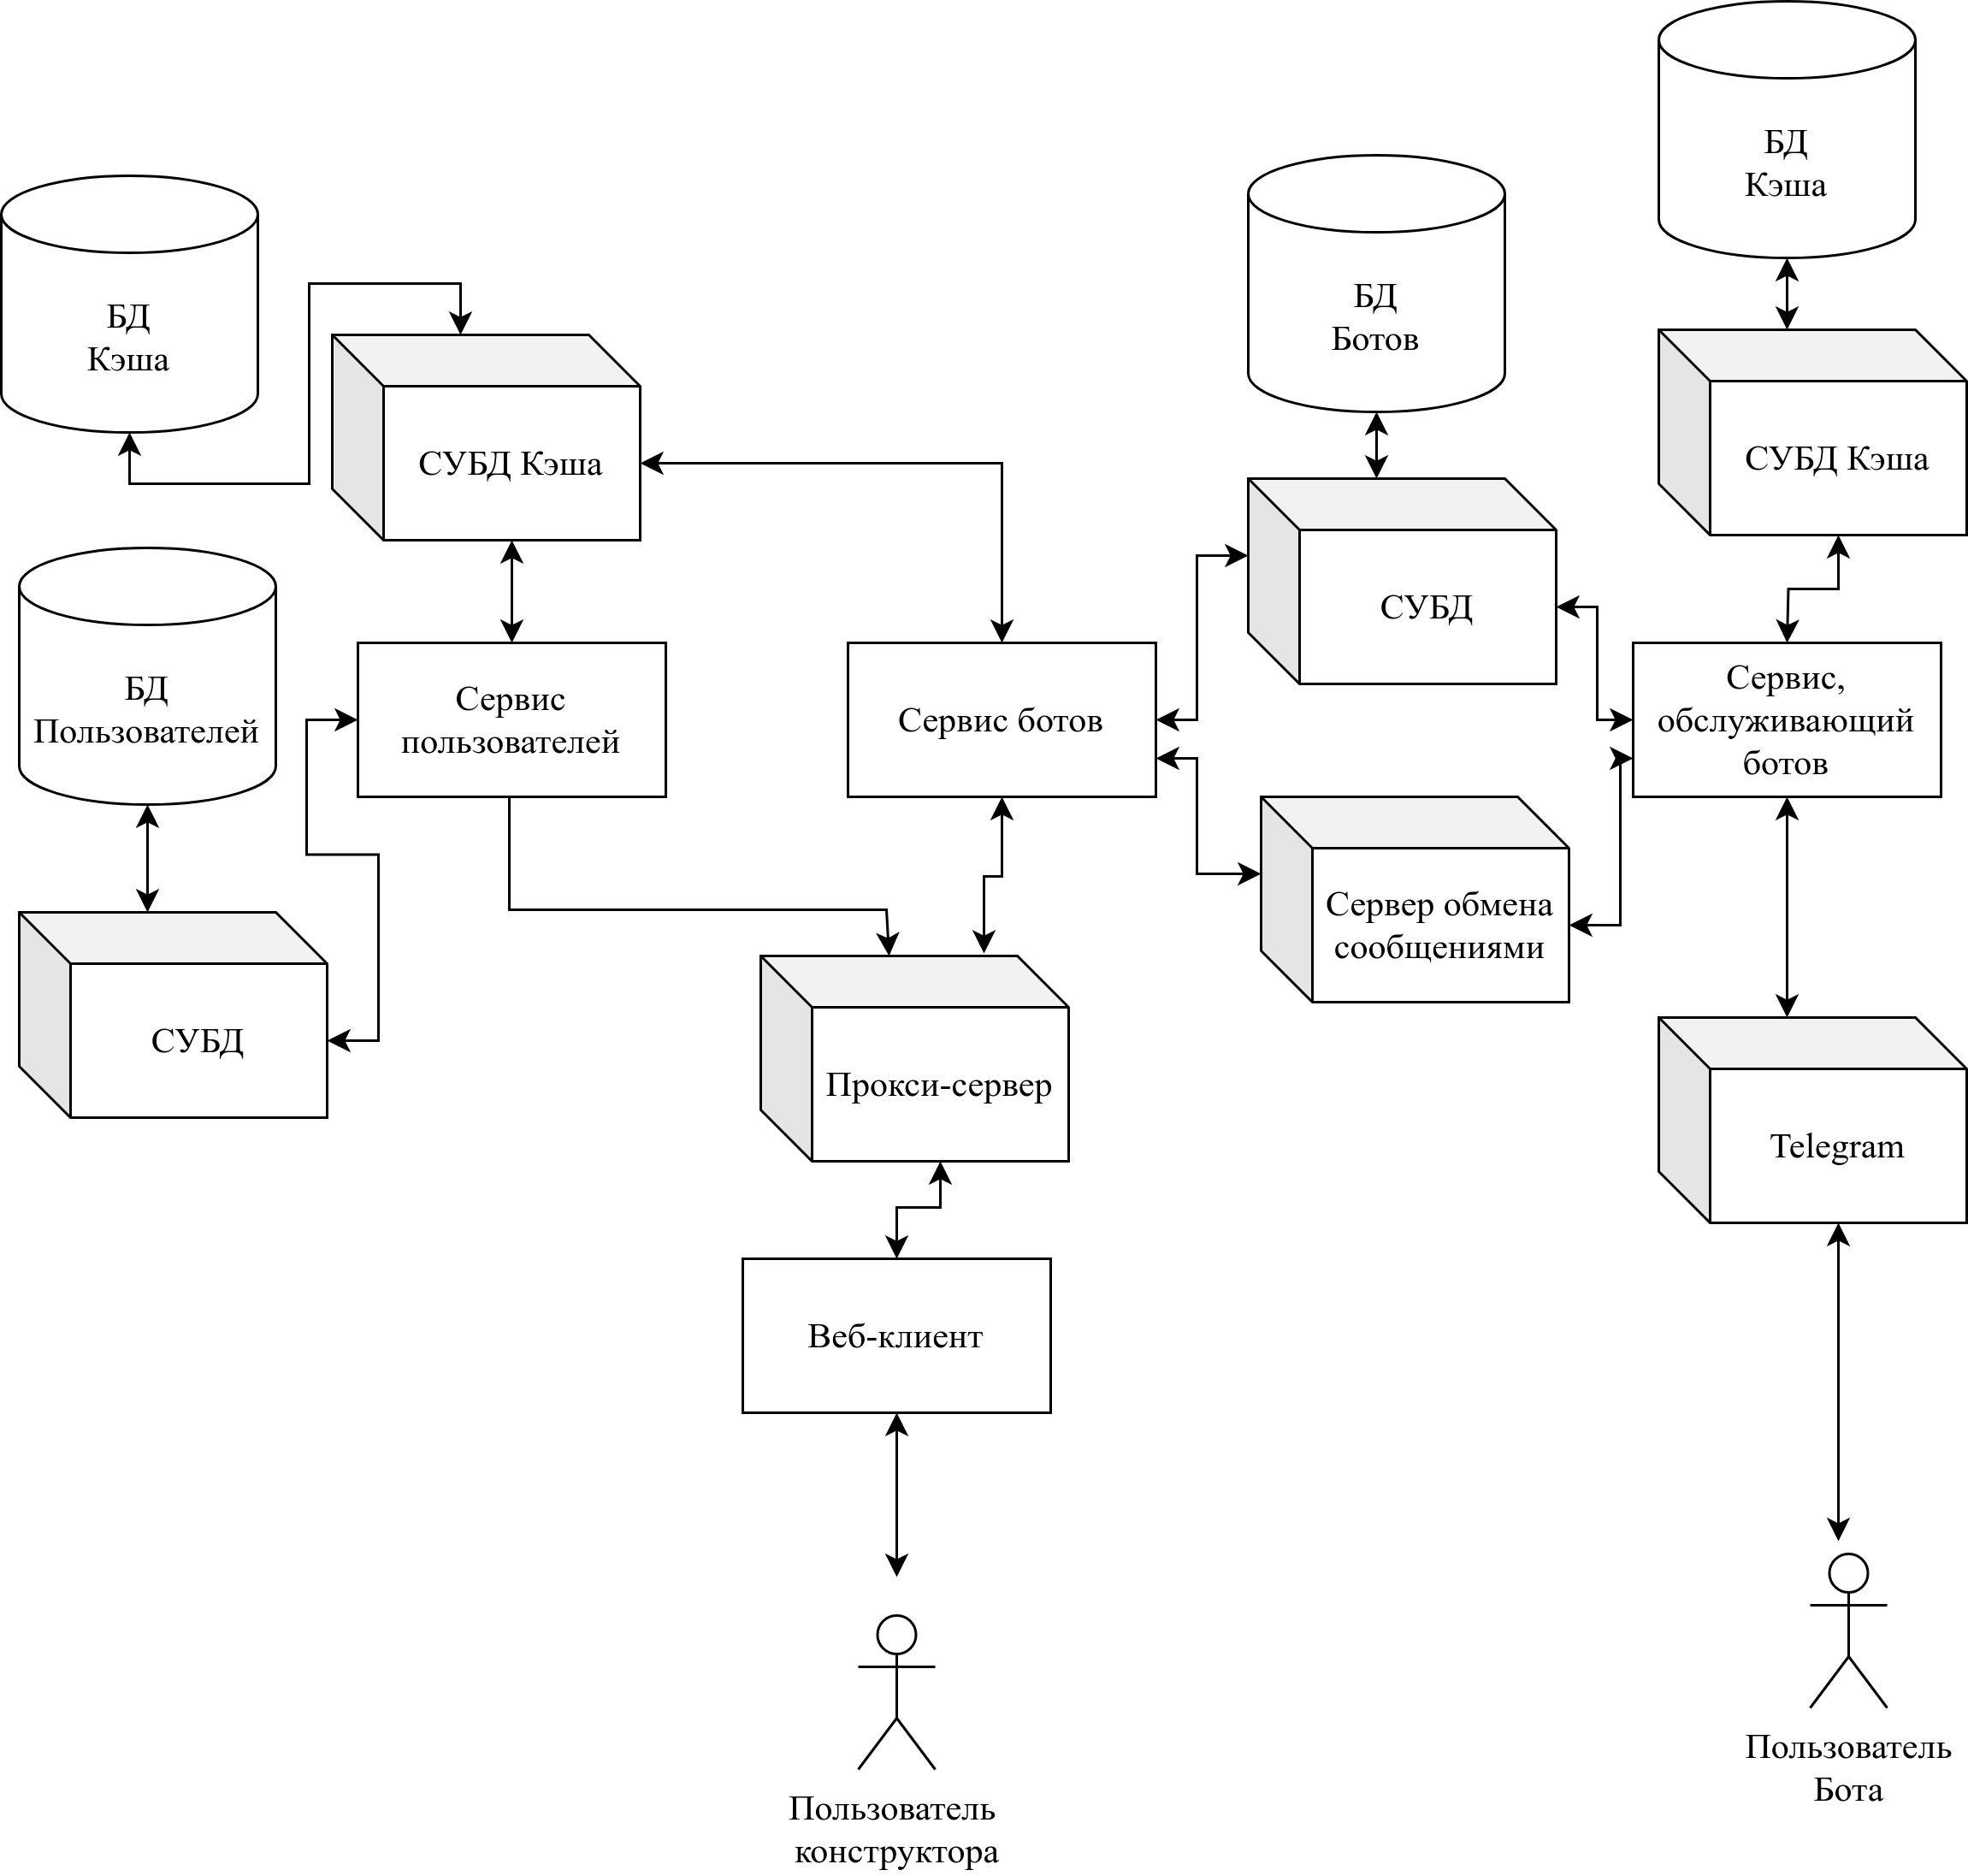
\includegraphics[width=0.95\textwidth]{structures/general}
	\caption{Общая структура конструктора}
	\label{f:general-struct}
\end{figure}


Конструктор состоит из серверной и клиентской части.

Серверная часть состоит из нескольких сервисов:
\begin{itemize}
	\item сервис пользователей;
	\item сервис ботов;
	\item сервис, обслуживающий ботов.
\end{itemize}

Сервис пользователей взаимодействует с хранилищами в виде базы
данных и кэша, в которых хранятся пользователи конструктора и их токены
авторизации. Через него происходит регистрация и аутентификация
пользователей.

Сервис ботов предоставляет программный интерфейс для работы с
ботами. Данный сервис выполняет следующие функции:
\begin{itemize}
	\item создание ботов;
	\item редактирование ботов;
	\item удаление ботов;
	\item запуск и остановка ботов.
\end{itemize}

Данные ботов сохраняются в базе данных. Авторизация пользователя
происходит с помощью данных из кэша пользователей.

Сервис, обслуживающий ботов, обрабатывает запросы от запущенных
Telegram ботов, также он получает и выполняет команды на запуск и
остановку ботов от сервиса ботов, команды при этом посылаются через сервер
обмена сообщениями. Данный сервис сохраняет и получает текущее состояние
пользователя из кэша.

Пользователь взаимодействует с конструктором через веб-интерфейс,
который через прокси-сервер связан с сервисами пользователей и ботов.
Веб-интерфейс является клиентской частью конструктора.


\subsection{Разработка структуры серверной части конструктора}


В данном разделе описываются разработанные структуры серверной части
конструктора и его основные алгоритмы функционирования.

\subsubsection{Модульная структура серверной части конструктора}

Модуль – набор структур и методов, который обобщает какую-то логику
приложения.

Модульная структура серверной части конструктора представлена на
рисунке~\ref{f:mod-server-struct}.

\begin{figure}[ht]
	\centering
	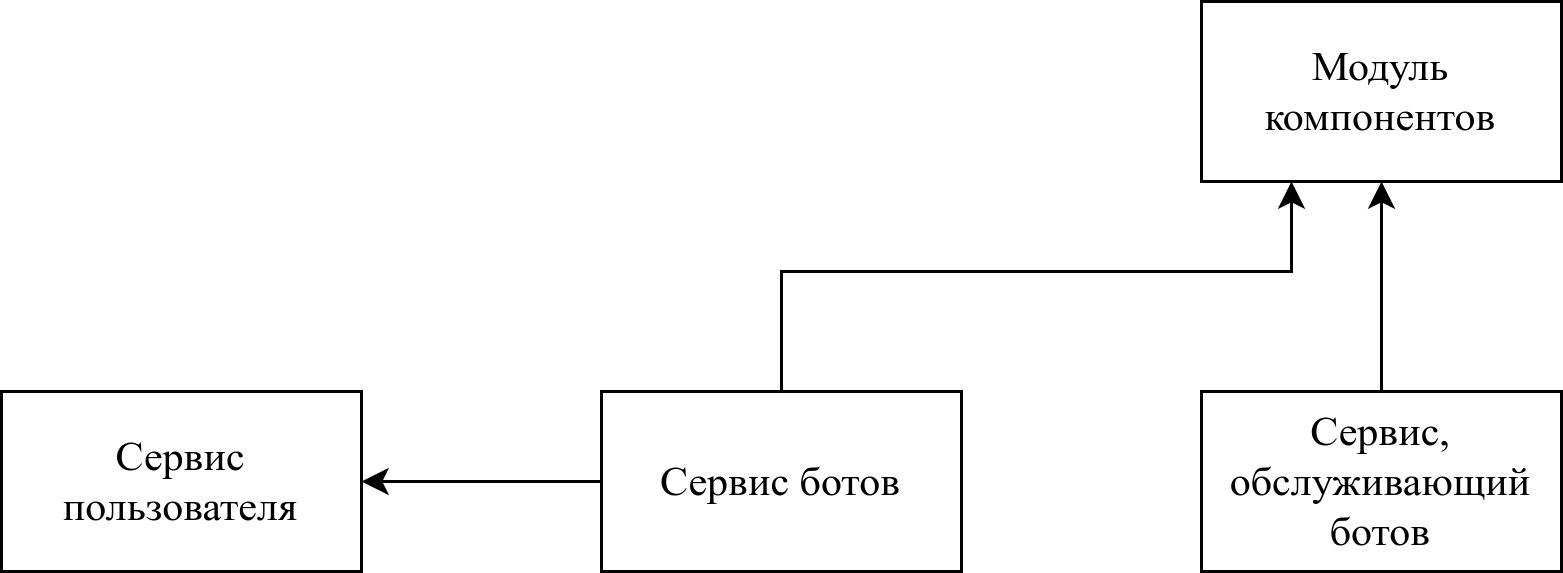
\includegraphics[width=0.8\textwidth]{structures/server/mod}
	\caption{Модульная структура серверной части конструктора}
	\label{f:mod-server-struct}
\end{figure}

Сервис ботов зависит от сервиса пользователей, который предоставляет
первому методы для авторизации пользователя. Также сервис ботов зависит
от модуля компонентов, который описывает структуры компонентов и
реализует их логику выполнения.

Для выполнения логики ботов сервис, обслуживающий ботов, вызывает
методы из модуля компонентов.

\subsubsection{Структура модуля компонентов}

Модуль компонентов состоит из следующих подмодулей:
\begin{itemize}
	\item подмодуль компонентов;
	\item подмодуль контекста;
	\item подмодуль исполнителя;
	\item подмодуль ввода-вывода.
\end{itemize}

Структура модуля компонентов представлена на рисунке~\ref{f:mod-comp-struct}.

\begin{figure}[ht]
	\centering
	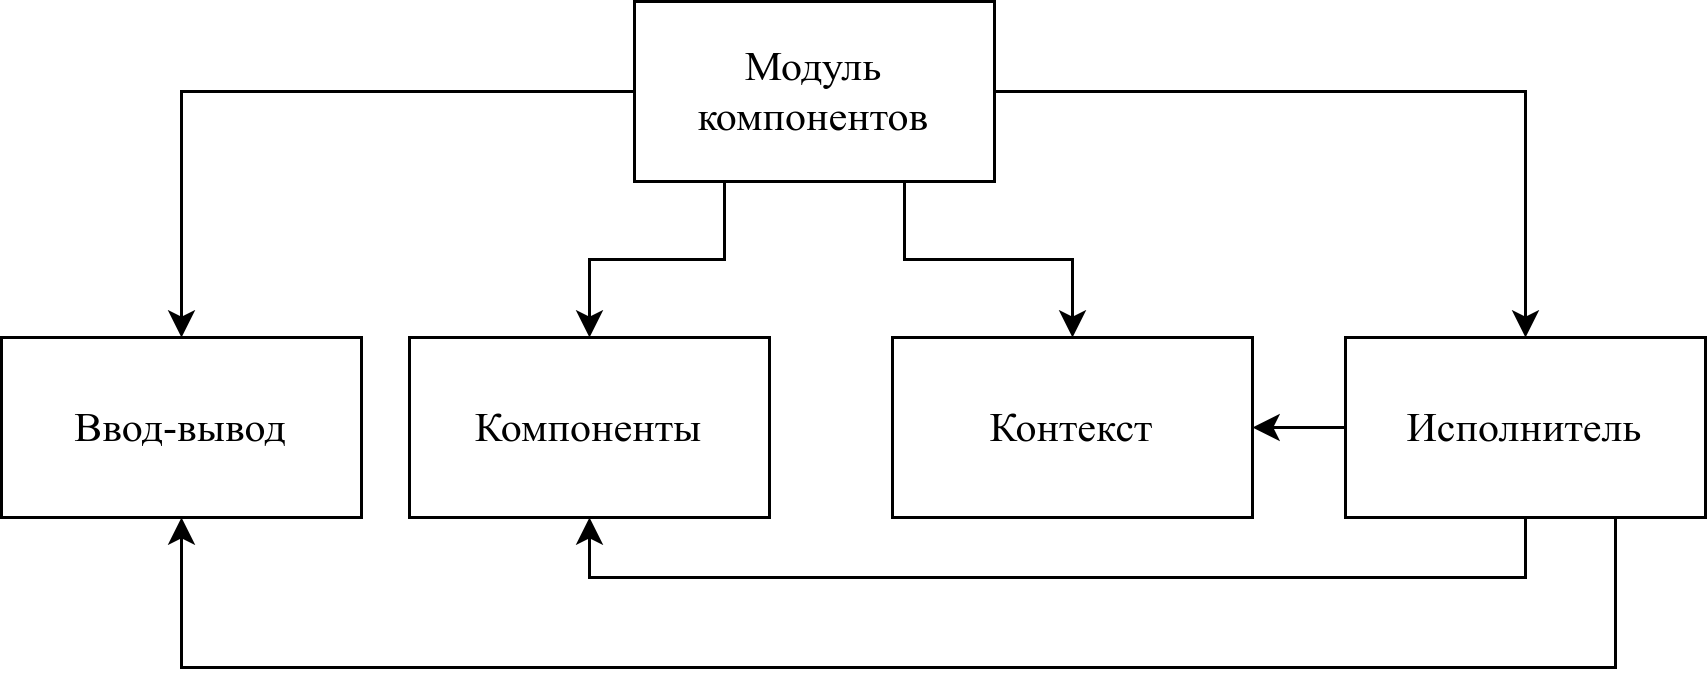
\includegraphics[width=0.8\textwidth]{structures/server/mod-comp}
	\caption{Структура модуля компонентов}
	\label{f:mod-comp-struct}
\end{figure}

Подмодуль компонентов содержит структуру и реализацию логики
компонентов. Каждый компонент реализует общий интерфейс компонента,
который определен в данном подмодуле.

В данном подмодуле определены следующие компоненты:
\begin{itemize}
	\item 	компонент ввода текста;
	\item 	компонент отправки сообщения;
	\item 	компонент вывода кнопок;
	\item 	компонент форматирования;
	\item 	компонент точки входа;
	\item 	компонент условия.
\end{itemize}

Подмодуль ввода-вывода предоставляет интерфейс, через который
окружение обменивается данными с рядом компонентов.

Подмодуль контекста содержит методы для работы с контекстом.
Контекст в рамках бота – память, с которой работают компоненты:
компоненты получают из контекста данные для выполнения и записывают в
него результат.

Исполнитель представляет собой объект, который содержит в себе
контекст и интерфейс ввода-вывода. Через него происходит выполнение
компонентов.


\subsubsection{Алгоритмы функционирования серверной части конструктора}

Пользователь конструктора взаимодействует с сервисом ботом, который
контролирует изменение данных и состояние ботов.
Схема алгоритма обработки запросов от пользователей сервиса ботов
представлен на рисунке~\ref{f:bot-service-alg}.

\begin{figure}[hp]
	\centering
	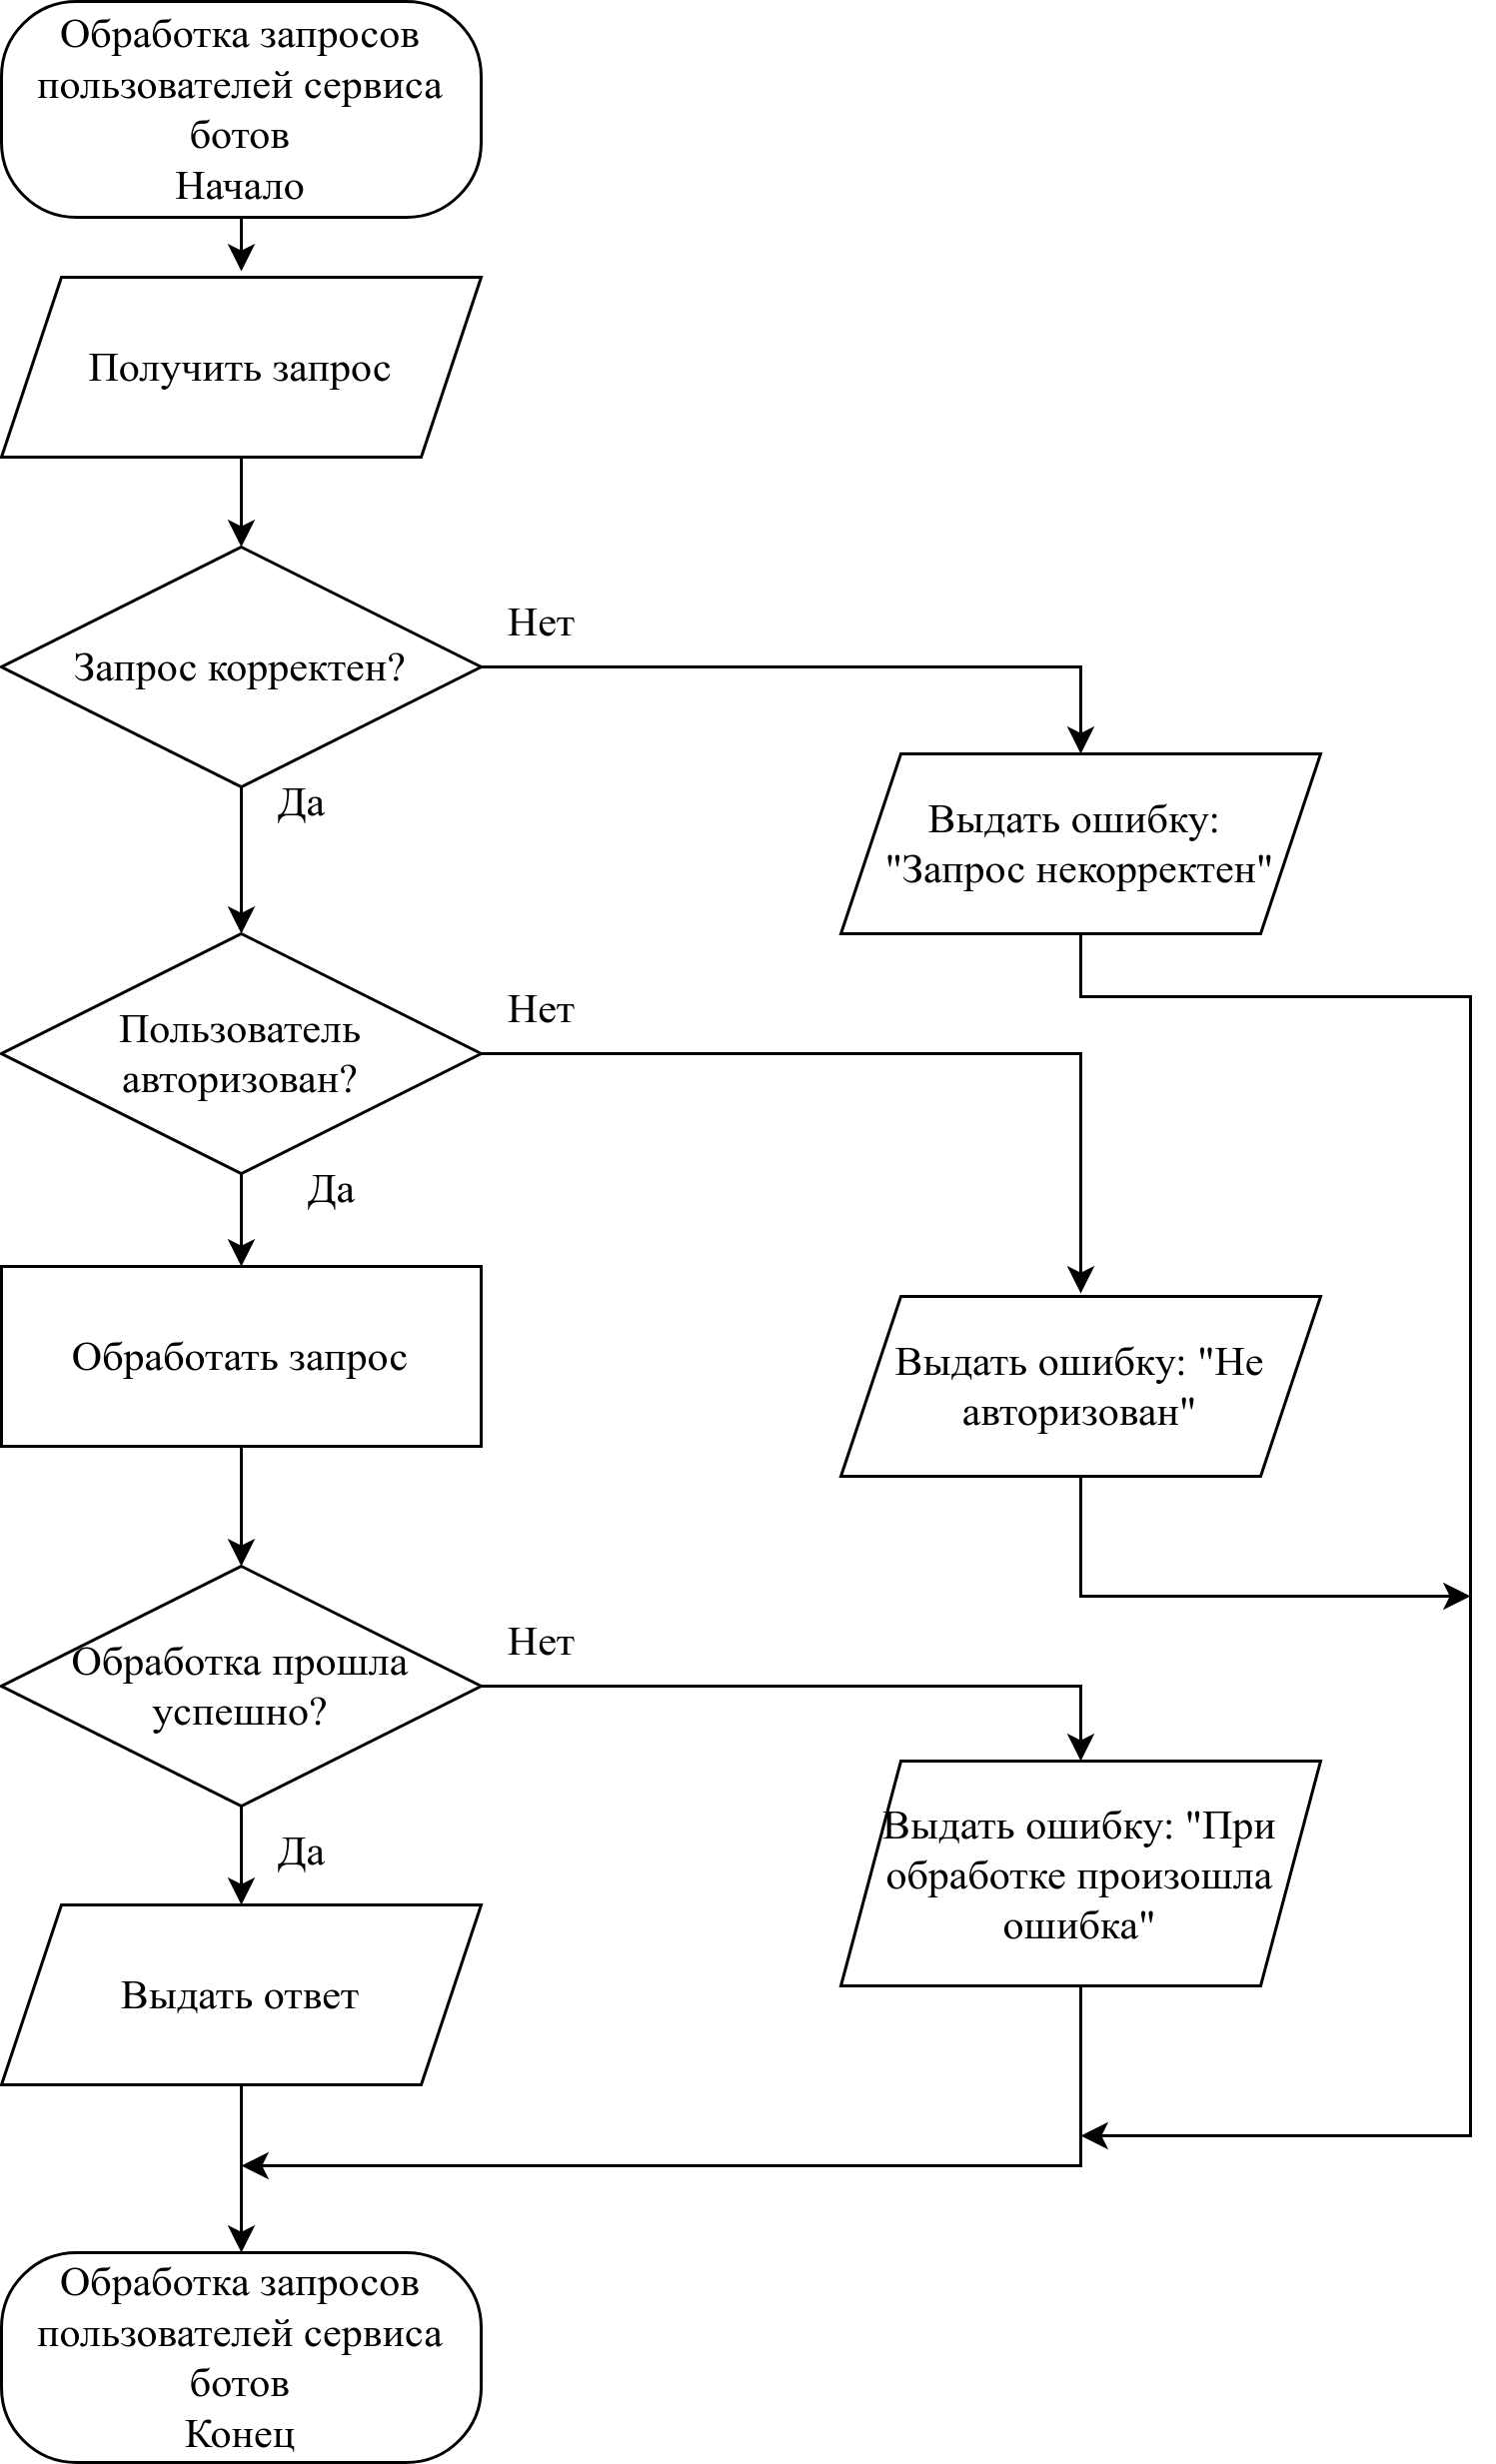
\includegraphics[height=0.9\textheight]{bot-service-alg}
	\caption{Схема алгоритма обработки запросов от пользователей сервиса ботов}
	\label{f:bot-service-alg}
\end{figure}

При получении запроса проверяется его корректность.
Если запрос не корректен, например, такое обращение не доступно, то
выводится соответствующая ошибка. Чтобы обработка прошла успешно, пользователь
должен быть авторизован в системе. В случае успешной обработки запроса выдается
ответ, иначе - ошибка.


При взаимодействии Telegram пользователя с ботом происходит
отправка запросов сервису, обслуживающему ботов, который в дальнейшем
обрабатывает данное событие. Схема алгоритма обработки запросов от
пользователя бота представлен на рисунке~\ref{f:bot-worker-alg}.


\begin{figure}[hp]
	\centering
	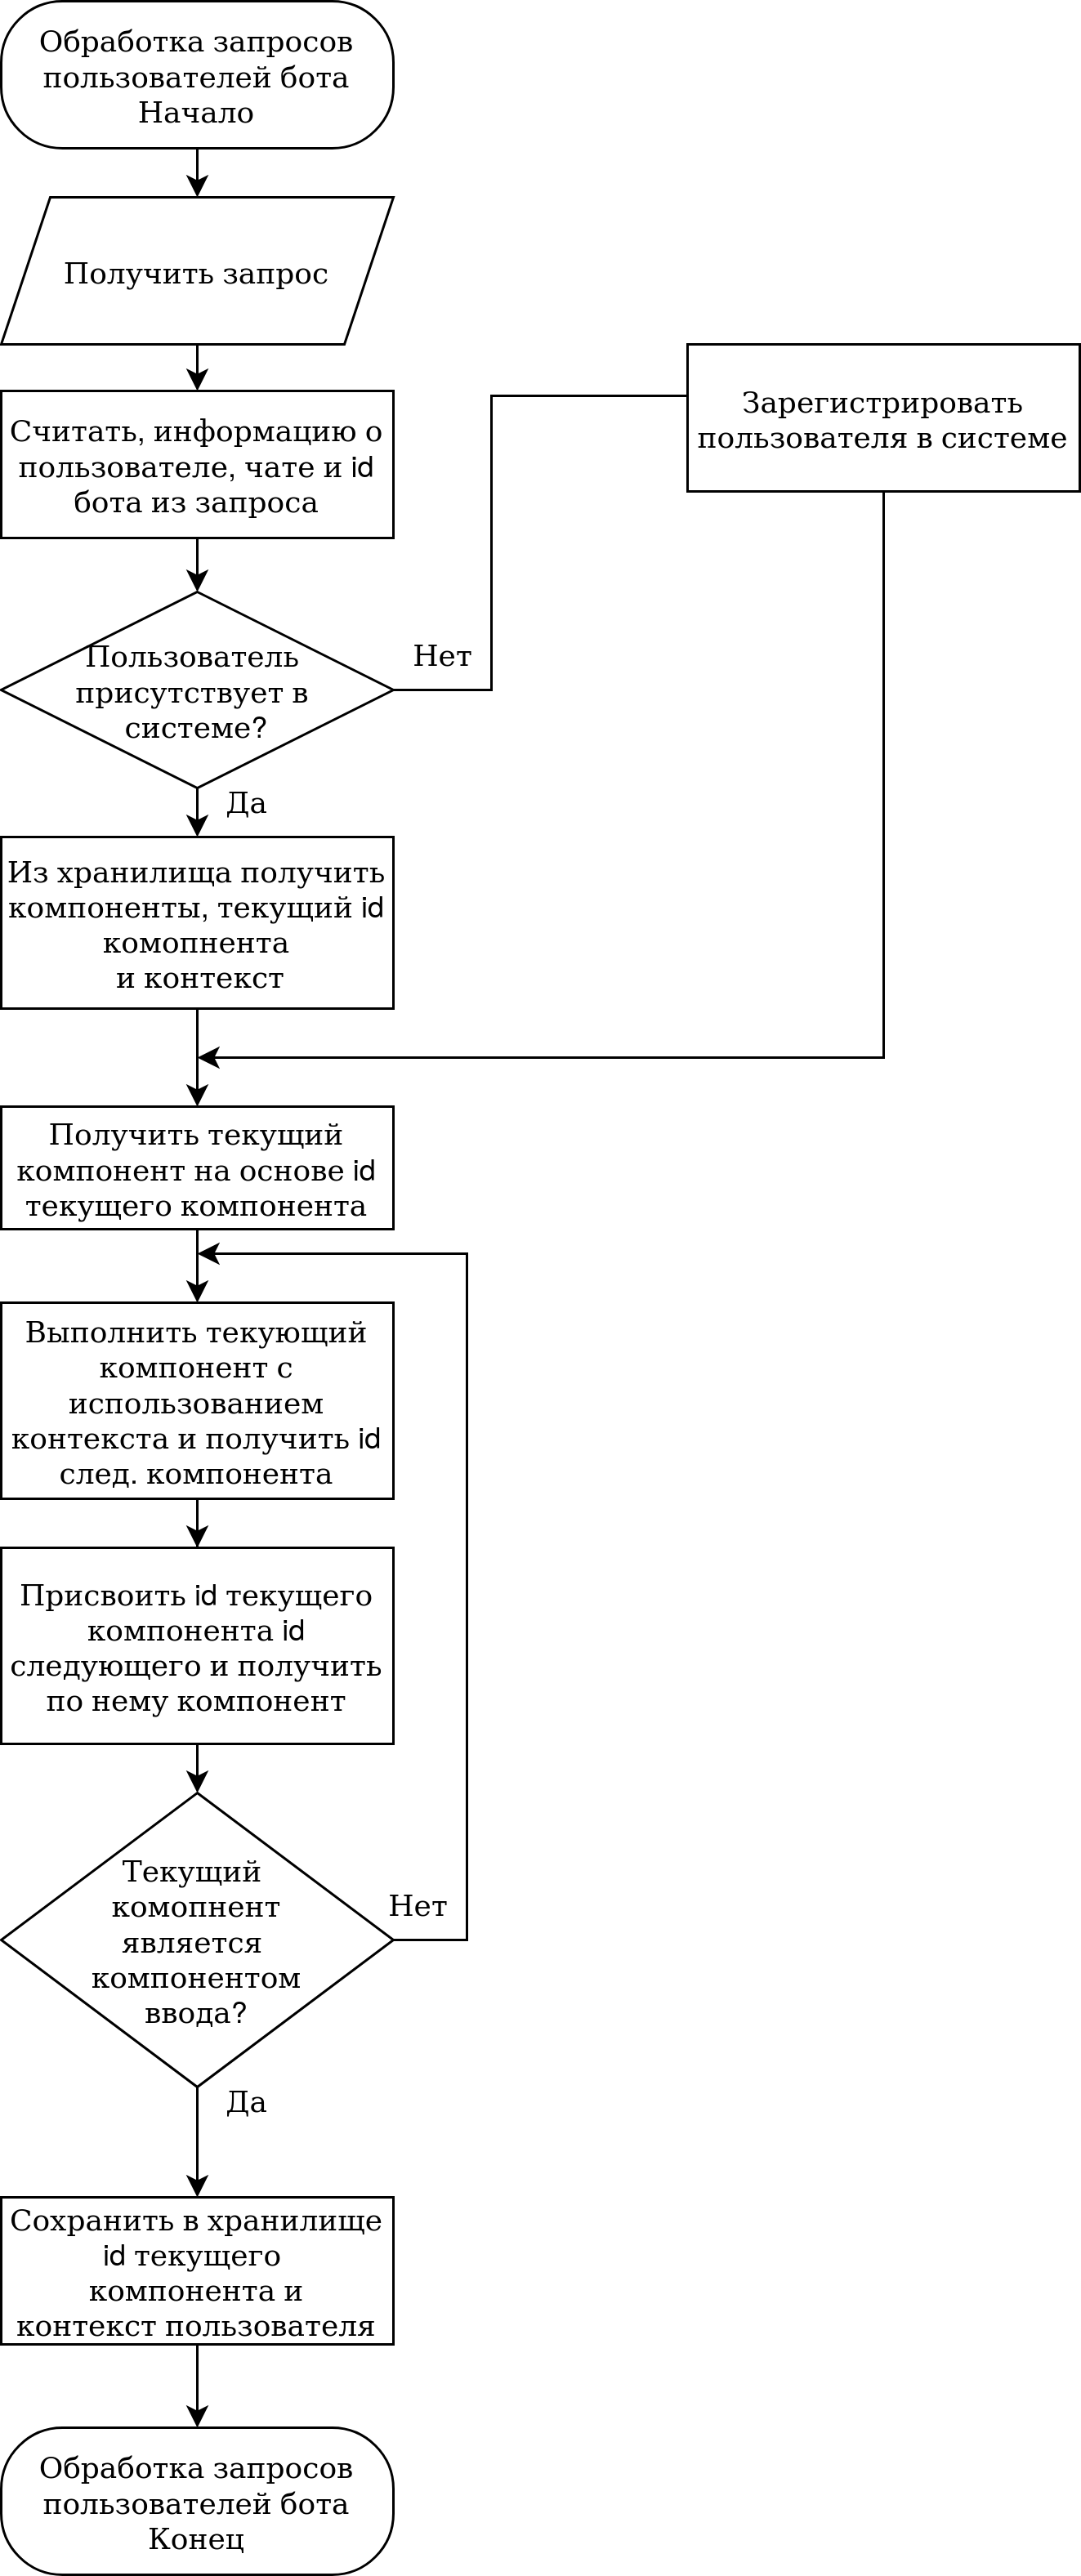
\includegraphics[height=0.9\textheight]{bot-worker-alg}
	\caption{Схема алгоритма обработки запросов от пользователей ботов}
	\label{f:bot-worker-alg}
\end{figure}

При принятии события сервисом происходит считывание следующих
данных:
\begin{itemize}
	\item информация о пользователе;
	\item информация о чате;
	\item id бота, от которого пришло сообщение.
\end{itemize}

На основе этих данных из хранилища идёт получение следующих
данных:
\begin{itemize}
	\item контекст пользователя;
	\item id текущего компонента пользователя;
	\item компонентов бота.
\end{itemize}

На основании id текущего компонента происходит получение текущего
компонента, который затем выполняется. Результат выполнения представляет
собой id следующего компонента, который присваивается текущему.

На основании следующего компонента принимается решение: если
компонент ожидает ввода каких-либо данных, то алгоритм заканчивается с
сохранением контекста и id текущего компонента, иначе идет выполнение
следующего компонента.

\newpage

\subsubsection{Обеспечение защиты информации клиентов конструктора}

\subsection{Разработка структуры клиентской части конструктора}


В данном разделе описываются разработанные структуры клиентской части
конструктора и его диаграммы состояний.

\subsubsection{Структура интерфейса конструктора}

Пользовательский интерфейс конструктора представляет собой
административную панель с набором следующих страниц:

\begin{itemize}
	\item страница аутентификации;
	\item страница регистрации;
	\item страница ботов пользователя конструктора;
	\item страница создания нового бота;
	\item страница запуска бота;
	\item страница редактирования бота.
\end{itemize}


Каждая страница состоит из верхней панели и содержимого страницы.
Верхняя панель содержит ссылки на страницы аутентификации и регистрации,
если пользователь не вошёл в систему, иначе - кнопку “выйти из системы”.

Страница аутентификации и регистрации содержат поля ввода логина и
пароля пользователя, под которым располагается кнопка входа или
регистрации. Шаблон содержимого страницы аутентификации представлен на
рисунке

\paragraph{Длинный длинный длиннный длинный длинный длиннный длинный длинный длинный текст}




{
\newcommand{\scale}{0.65}

\section{Расчёт координат объектов визуального редактора}


Область редактора представляет собой координатную плоскость,
на которой располагаются компоненты бота.
Расположение компонента обеспечивается координатами $ ( x_c , y_c ) $,
которые указывают
на левый верхний угол компонента.

При перемещении компонента вычисляются смещения
$ \bigtriangleup x $ и $\bigtriangleup y$
относительно координат нажатой мыши
$ (x_m, y_m) $ по формулам
\begin{gather}
	\bigtriangleup x = x_c - x_m, \\
	\bigtriangleup y = y_c - y_m.
\end{gather}

Данные смещения используются для расчёта новых координат компонента
$ (x_c', y_c') $ при перемещении мыши с координатами
$ (x_m', y_m') $,
которые вычисляются по формулам
\begin{gather}
	x_c' = x_m' - \bigtriangleup x, \\
	y_c' = y_m' - \bigtriangleup y.
\end{gather}

Расположение компонента на координатной плоскости показано
на рисунке~\ref{f:component-crds}.

\begin{figure}[h]
	\centering
	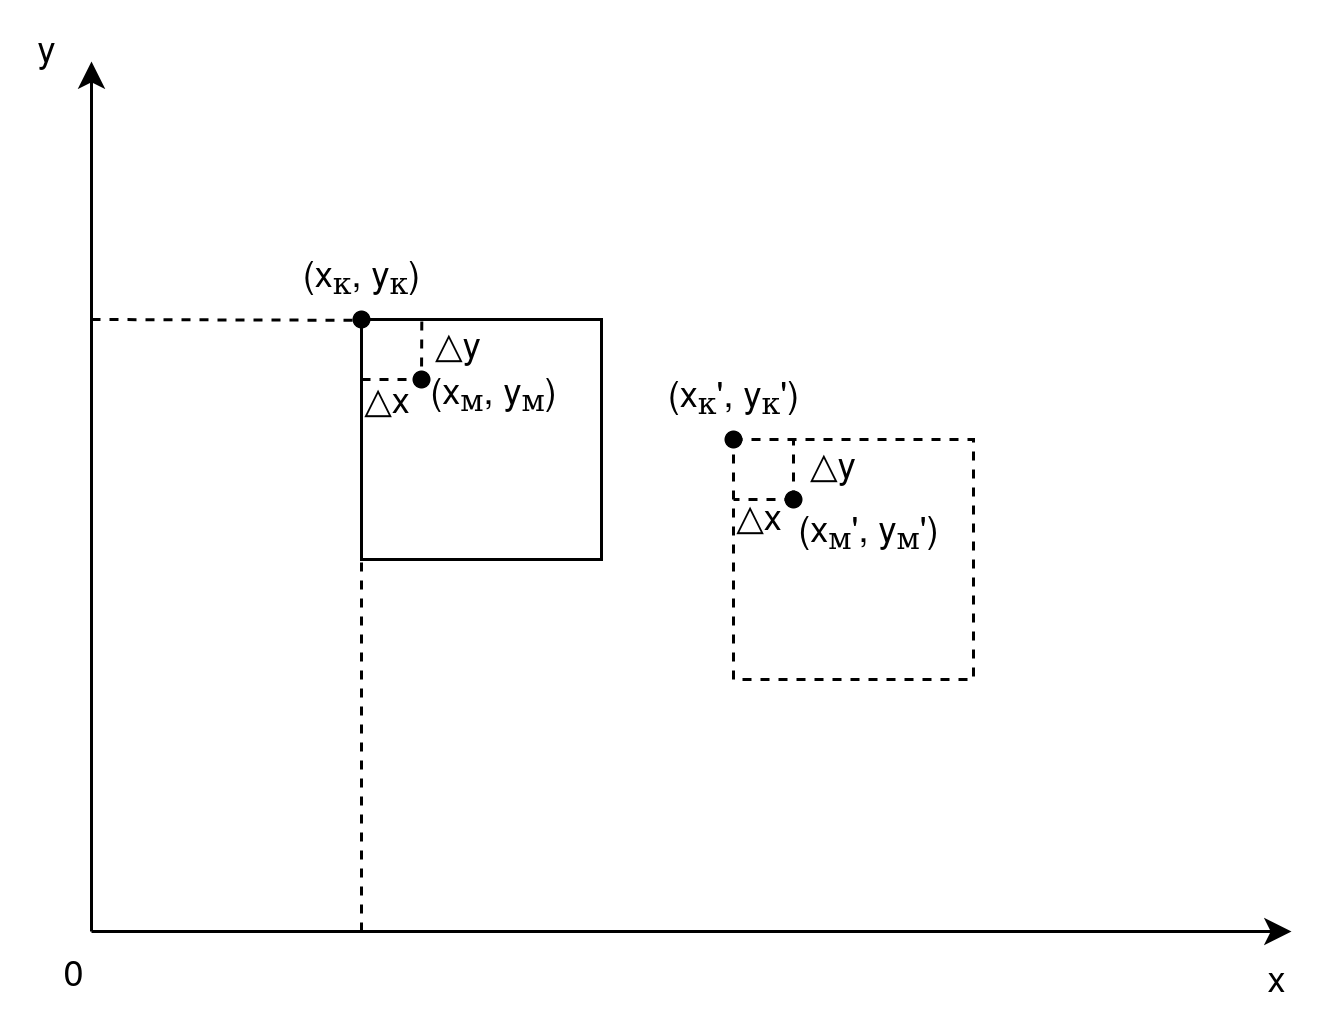
\includegraphics[width=\scale\textwidth]{component-crds}
	\caption{Координаты расположения компонентов}
	\label{f:component-crds}
\end{figure}

Связи между компонентами представляют собой линию со стрелкой.
Линия имеет координаты начала
$ (x_{out}, y_{out}) $
и конца
$ (x_{in}, y_{in}) $, которые представляют собой точки центра окружностей
соединительных точек выхода и входа компонентов.
Расположение связей компонентов на координатной плоскости показано на
рисунке~\ref{f:line-crds}.

\begin{figure}[h]
	\centering
	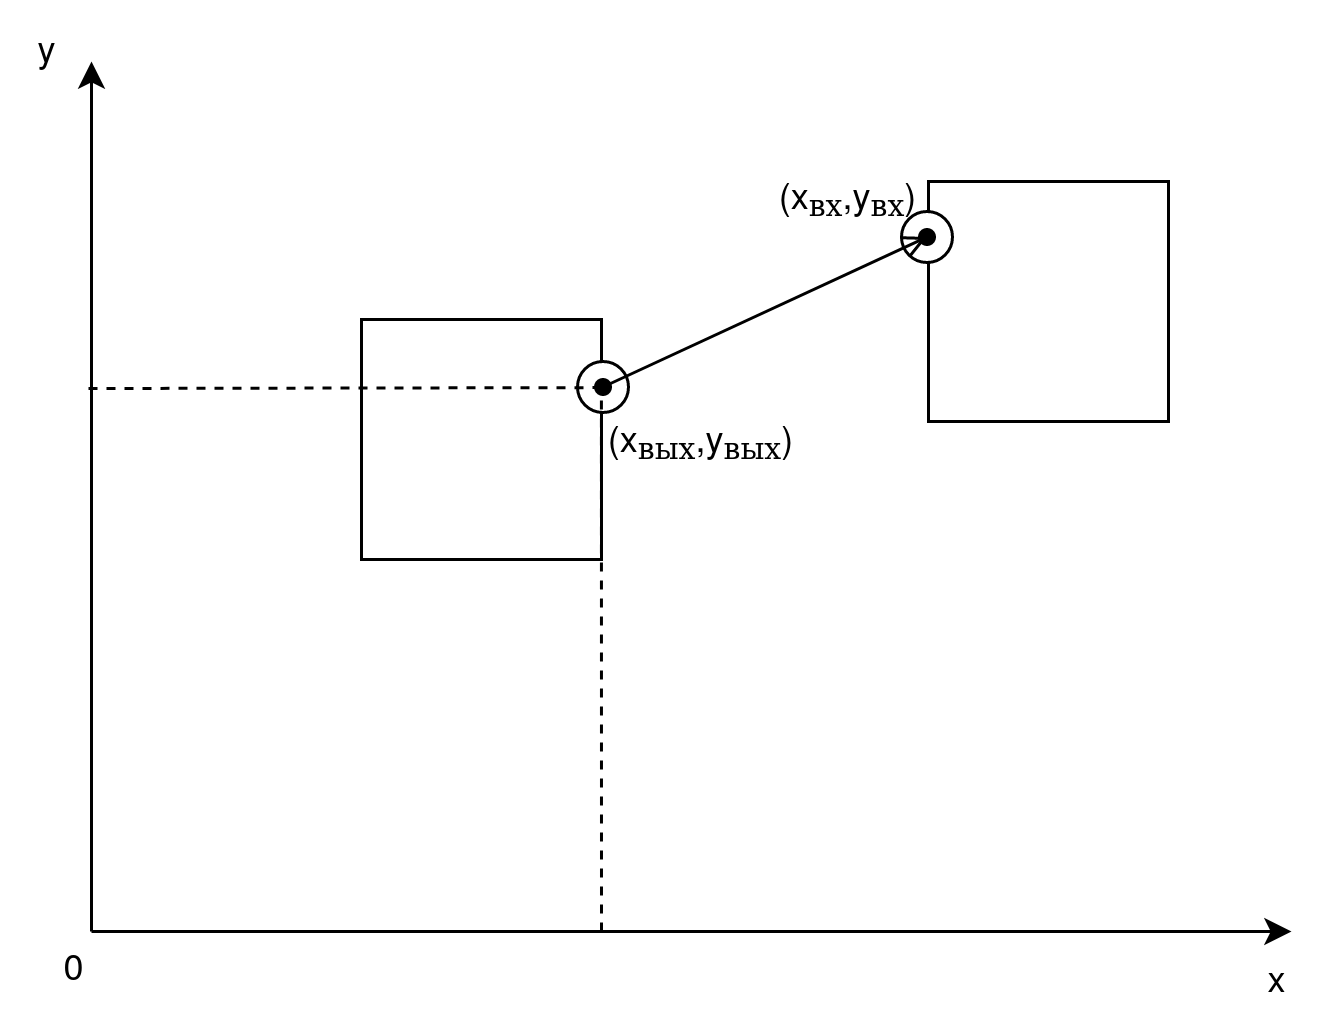
\includegraphics[width=\scale\textwidth]{line-crds}
	\caption{Координаты расположения связей компонентов}
	\label{f:line-crds}
\end{figure}

Стрелка представляет собой две примыкающих к линии прямых.
Стрелка имеет длину
$ a $ и угол между примыкающих прямых $ \alpha $.

Линия между компонентами наклонена под углом $ \beta $ относительно оси $ y $. Угол
вычисляется по формуле
\begin{equation}
	\beta = \arctan(\frac{x_{in} - x_{out}}{y_{in} - y_{out}}).
\end{equation}

Точка
$ (x_a, y_a) $ является окончанием стрелки и её координаты вычисляются по формулам
\begin{gather}
	x_a = x_{in} - sin \beta * a, \\
	y_a = y_{in} - cos \beta * a.
\end{gather}


Расчет смещения $b$ примыкающих прямых относительно основной линии и
смещений $\bigtriangleup x_a$
и $\bigtriangleup y_a$ относительно осей $x$ и $y$ происходит по формулам
\begin{gather}
	b = \tan(\frac{\alpha}{2})*a, \\
	\bigtriangleup x_a = \cos(\beta) * b, \\
	\bigtriangleup y_a = \sin{\beta} * b.
\end{gather}


Сами точки окончания примыкающих прямых
$ (x_{a1}, y_{a1}) $ и $ (x_{a2}, y_{a2}) $
вычисляются по формулам
\begin{gather}
	x_{a1} = x_a + \bigtriangleup x_a, \\
	y_{a1} = y_a - \bigtriangleup y_a, \\
	x_{a2} = x_a - \bigtriangleup x_a, \\
	y_{a2} = y_a + \bigtriangleup y_a.
\end{gather}

Расположение стрелки на координатной плоскости представлено
на рисунке~\ref{f:arrow-crds}.

\begin{figure}[h]
	\centering
	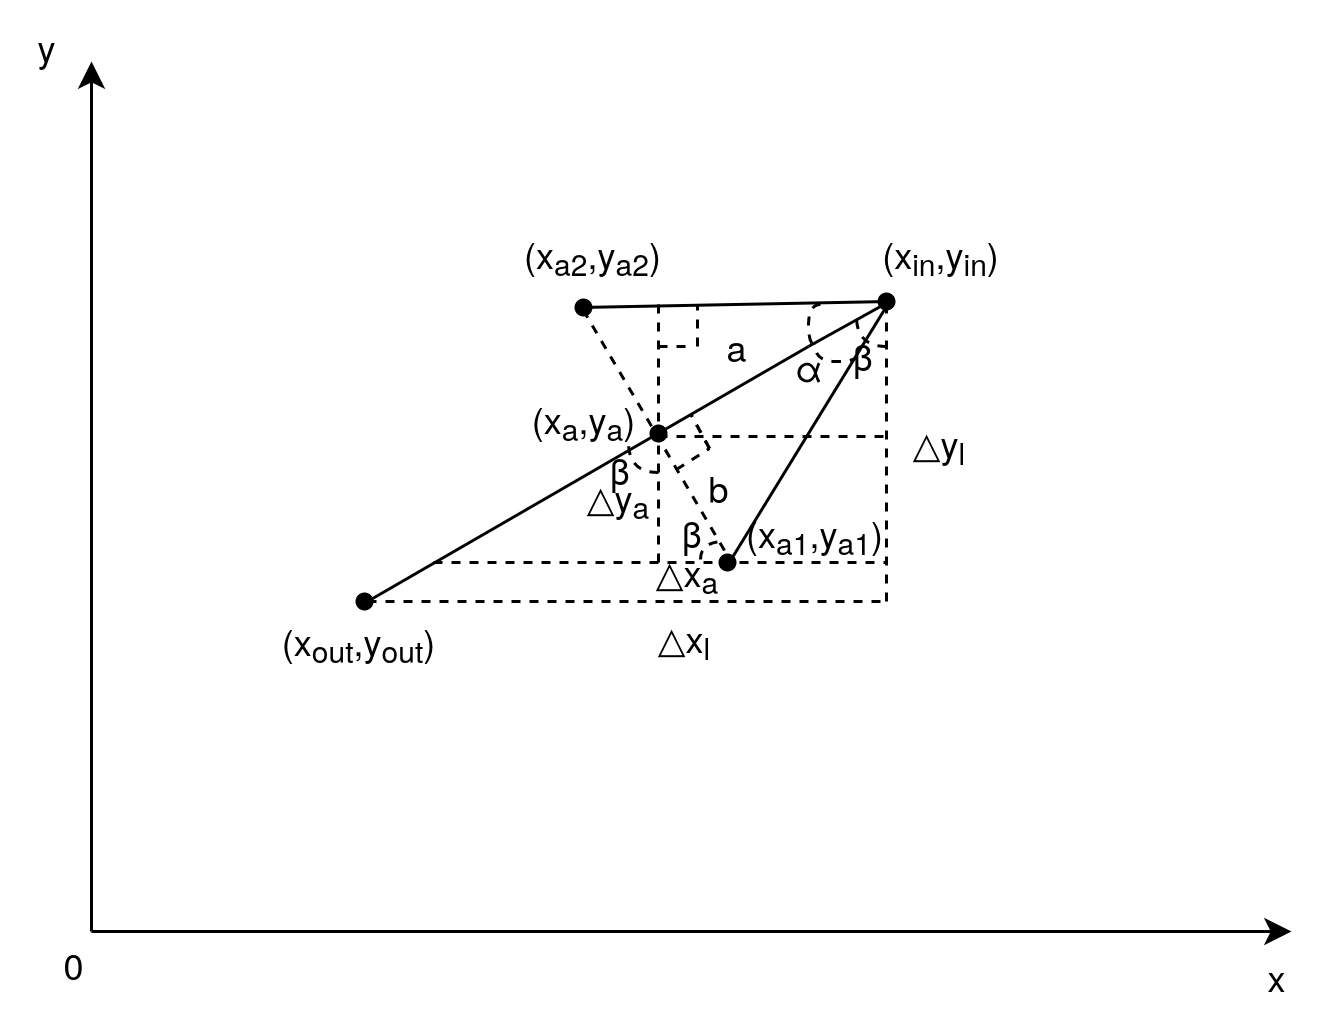
\includegraphics[width=\scale\textwidth]{arrow-crds}
	\caption{Координаты расположения стрелки}
	\label{f:arrow-crds}
\end{figure}


}




\end{document}
